% Compile from this folder:
% pdflatex -interaction=nonstopmode -halt-on-error group_4_presentation.tex
\documentclass[aspectratio=169,10pt,t]{beamer}
\usepackage[T1]{fontenc}
\usepackage{helvet}
\usepackage{appendixnumberbeamer}
\usepackage{booktabs,amsmath,array,tabularx,tikz,ragged2e}
\graphicspath{{../figures/}}
\usetikzlibrary{arrows.meta,positioning,calc}
\renewcommand{\tabularxcolumn}[1]{>{\RaggedRight\arraybackslash}p{#1}}
\newcolumntype{P}[1]{>{\RaggedRight\arraybackslash}p{#1}}
\renewcommand{\familydefault}{\sfdefault}
\definecolor{slate}{cmyk}{.4,.2,0,.6}
\definecolor{footerblue}{cmyk}{.54903,.31374,0,.45097}
\definecolor{ink}{cmyk}{0,0,0,1}
\definecolor{institute}{cmyk}{0,1,1,0}
\definecolor{pale}{RGB}{242,246,249}
\usetheme{default}
\setbeamercolor{normal text}{fg=ink,bg=white}
\setbeamercolor{structure}{fg=slate}
\setbeamercolor{frametitle}{fg=slate,bg=white}
\setbeamerfont{frametitle}{size=\fontsize{12}{14}\selectfont,series=\bfseries}
\setbeamertemplate{navigation symbols}{}
\setbeamertemplate{itemize item}{\color{ink}\scriptsize$\blacktriangleright$}
\setbeamertemplate{frametitle}{\vspace{.52cm}\raggedright\insertframetitle\par\vspace{.20cm}}
\setbeamersize{text margin left=1cm,text margin right=1cm}
\setbeamertemplate{footline}{%
\leavevmode\hbox to\paperwidth{%
\hspace{1cm}%
{\color{footerblue}\fontsize{7}{8.4}\selectfont
Efficient LLM Serving on a Single GPU}%
\hfill%
{\color{footerblue}\fontsize{7}{8}\selectfont
\hspace{.45cm}\insertframenumber\,/\,\inserttotalframenumber}%
\hspace{1cm}%
}%
\vspace{.70cm}%
}
\hypersetup{colorlinks=true,urlcolor=footerblue,linkcolor=footerblue,pdfauthor={Vishank Singh; Anup Chavan},pdftitle={Efficient LLM Serving on a Single GPU}}
\linespread{1.02}
\setlength{\parskip}{.22em}
\newenvironment{points}{\raggedright\begin{itemize}\setlength{\itemsep}{.46em}}{\end{itemize}}
\newcommand{\src}[1]{\vfill{\fontsize{7}{8.4}\selectfont\color{footerblue}Source: #1\par}}
\newcommand{\smallnote}[1]{{\fontsize{9}{10.8}\selectfont #1\par}}
\tikzset{box/.style={draw=slate,line width=.7pt,fill=pale,align=center,minimum height=.85cm,text width=2.55cm,font=\small,inner sep=5pt},arr/.style={-{Latex[length=2mm]},line width=.8pt,draw=slate},lab/.style={font=\scriptsize,align=center,text=slate}}

% Uniform table formatting; scoped so surrounding text retains its size.
\BeforeBeginEnvironment{tabular}{\begingroup\fontsize{7.6}{8.5}\selectfont\renewcommand{\arraystretch}{1.02}\setlength{\tabcolsep}{5pt}}
\AfterEndEnvironment{tabular}{\endgroup}
\BeforeBeginEnvironment{tabularx}{\begingroup\fontsize{7.6}{8.5}\selectfont\renewcommand{\arraystretch}{1.02}\setlength{\tabcolsep}{5pt}}
\AfterEndEnvironment{tabularx}{\endgroup}

% Slightly smaller body type with a little more leading.
\makeatletter
\renewcommand\normalsize{\@setfontsize\normalsize{9.5}{12}}
\makeatother
\AtBeginDocument{\normalsize}
\definecolor{mal}{RGB}{170,40,40}
\definecolor{ben}{RGB}{30,110,70}
\newcommand{\ins}[2]{{\color{#1}\bfseries #2}}
\begin{document}

\begin{frame}[plain,c]
\vspace{.75cm}

\begin{center}
{\normalsize\bfseries Group 4\par}
\vspace{.35cm}
{\fontsize{18}{21}\selectfont\bfseries Efficient LLM Serving\par}

\vspace{.35cm}
{\large Problem and Proposed Approach\par}

\vspace{.45cm}
{\fontsize{12}{14}\selectfont\bfseries Project 24: Quantisation, Prefix Caching and Speculative Decoding\par}

\vspace{.25cm}
\hrule height 1.2pt
\end{center}

\vspace{.35cm}
\begin{center}
\begin{tabular}{@{}ll@{}}
Vishank Singh & AI23BTECH11032\\[.15cm]
Anup Chavan & CS23BTECH11005
\end{tabular}\par
\end{center}

\vfill

\begin{center}
{\small 16 October 2026\par}
\end{center}
\end{frame}

\begin{frame}{LLM serving basics}
\centering
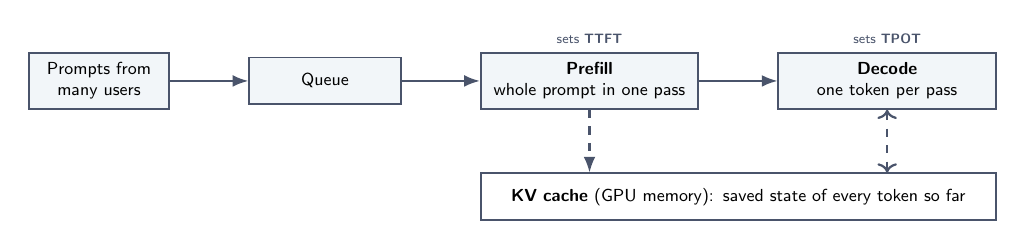
\begin{tikzpicture}[scale=.70,transform shape]
\node[box,text width=2.2cm] (req) at (0,0) {Prompts from\\many users};
\node[box,text width=2.4cm] (q) at (4.1,0) {Queue};
\node[box,text width=3.6cm] (pre) at (8.9,0) {\textbf{Prefill}\\whole prompt in one pass};
\node[box,text width=3.6cm] (dec) at (14.3,0) {\textbf{Decode}\\one token per pass};
\node[box,text width=9cm,fill=white] (kv) at (11.6,-2.1) {\textbf{KV cache} (GPU memory): saved state of every token so far};
\draw[arr](req)--(q);\draw[arr](q)--(pre);\draw[arr](pre)--(dec);
\draw[arr,dashed](pre.south)--++(0,-.6)-|([xshift=-2.7cm]kv.north);
\draw[arr,dashed,<->](dec.south)--++(0,-.6)-|([xshift=2.7cm]kv.north);
\node[lab,above=.05cm of pre] {sets \textbf{TTFT}};
\node[lab,above=.05cm of dec] {sets \textbf{TPOT}};
\end{tikzpicture}
\par\raggedright\vspace{.15cm}
\begin{points}
\item \textbf{TTFT}: time to first token (queue + prefill). \textbf{TPOT}: time per output token after that.
\item \textbf{Throughput}: requests finished per second.
\item Decode re-reads all weights for every token, so it is limited by memory bandwidth. Prefill is limited by compute.
\end{points}
\end{frame}

\begin{frame}{Problem}
\begin{points}
\item Default vLLM on one GPU is slower than it could be. Known fixes are smaller weights, a smaller KV cache, reuse of shared prompt prefixes and several tokens per pass.
\item Quantisation frees memory, but a draft model for speculative decoding uses memory and GPU time.
\item Whether a fix helps depends on load, prompt length and prompt reuse.
\end{points}
\vspace{.12cm}
\centering
\begin{tabularx}{\linewidth}{@{}P{1.2cm}P{4.3cm}X@{}}
\toprule
Milestone & Scope & Expected outcome\\
\midrule
M1 & Quantised weights, FP8 KV cache, batching on one GPU & Measured gain over default vLLM at a latency target, quality kept\\
M2 & Prefix caching, speculative decoding & Conditions where each helps; load where speculation stops paying\\
M3 & All combined & Contribution of each technique; limiting resource; regimes where the setup is wrong\\
\bottomrule
\end{tabularx}\par
\end{frame}

\begin{frame}{Techniques}
\begin{tabularx}{\linewidth}{@{}P{2.6cm}XP{3.2cm}P{3.2cm}@{}}
\toprule
Technique & Idea & Bottleneck & vLLM flag\\
\midrule
AWQ & 4-bit weights instead of 16-bit & Memory bandwidth in decode & \texttt{--quantization awq}\\[.06cm]
FP8 KV cache & 8-bit KV cache; about twice as many tokens fit & KV-cache capacity & \texttt{--kv-cache-dtype fp8}\\[.06cm]
Prefix caching & Reuse KV cache of a prompt prefix seen before & Prefill compute & \texttt{--enable-prefix-caching}\\[.06cm]
Speculative decoding & 0.5B draft guesses 5 tokens; 3B model verifies them in one pass & Idle compute in decode & \texttt{--speculative-config}\\
\bottomrule
\end{tabularx}\par
\vspace{.2cm}
\begin{points}
\item Speculative decoding keeps the output unchanged; the 3B model verifies every token.
\item AWQ changes the weights, so output quality needs a separate check.
\end{points}
\end{frame}

\begin{frame}{Approach}
\centering
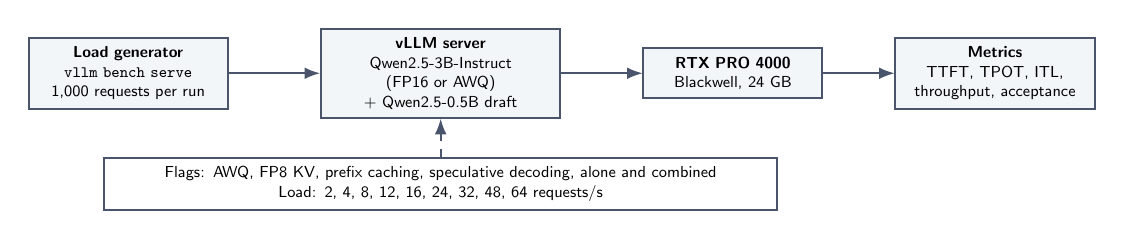
\begin{tikzpicture}[scale=.64,transform shape]
\node[box,text width=3.6cm] (gen) at (0,0) {\textbf{Load generator}\\\texttt{vllm bench serve}\\1,000 requests per run};
\node[box,text width=4.4cm] (srv) at (6.2,0) {\textbf{vLLM server}\\Qwen2.5-3B-Instruct\\(FP16 or AWQ)\\+ Qwen2.5-0.5B draft};
\node[box,text width=3.2cm] (gpu) at (12.0,0) {\textbf{RTX PRO 4000}\\Blackwell, 24 GB};
\node[box,text width=3.6cm] (met) at (17.2,0) {\textbf{Metrics}\\TTFT, TPOT, ITL,\\throughput, acceptance};
\draw[arr](gen)--(srv);\draw[arr](srv)--(gpu);\draw[arr](gpu)--(met);
\node[box,text width=13cm,fill=white] (grid) at (6.2,-2.2) {Flags: AWQ, FP8 KV, prefix caching, speculative decoding, alone and combined\\Load: 2, 4, 8, 12, 16, 24, 32, 48, 64 requests/s};
\draw[arr,dashed](grid.north)--(srv.south);
\end{tikzpicture}
\par\raggedright\vspace{.15cm}
\begin{points}
\item Each technique alone, then in combination, to separate individual effects from interactions.
\item Load from light to far past capacity.
\item Workload: 1,024 prompt + 128 output tokens per request.
\item 6 repeats per setting; about 560 runs over 4 days.
\end{points}
\end{frame}

\begin{frame}{Results: throughput limit}
\centering
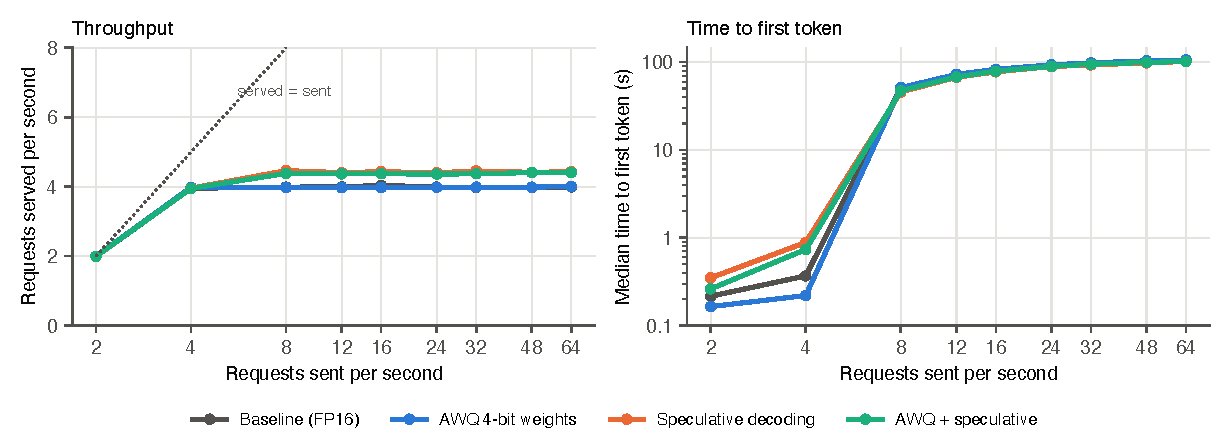
\includegraphics[width=.70\linewidth]{saturation.pdf}
\par\raggedright\vspace{.05cm}
\begin{points}
\item Up to 4 requests/s, every request is served and TTFT is 0.2--0.9 s.
\item Above that, the server finishes 4.0--4.4 requests/s and the rest queue; TTFT reaches 50--106 s.
\item No technique moves this limit much. Likely cause: prefill compute (about 4,000 prompt tokens/s), still to be profiled.
\end{points}
\end{frame}

\begin{frame}{Results: below the limit}
\centering
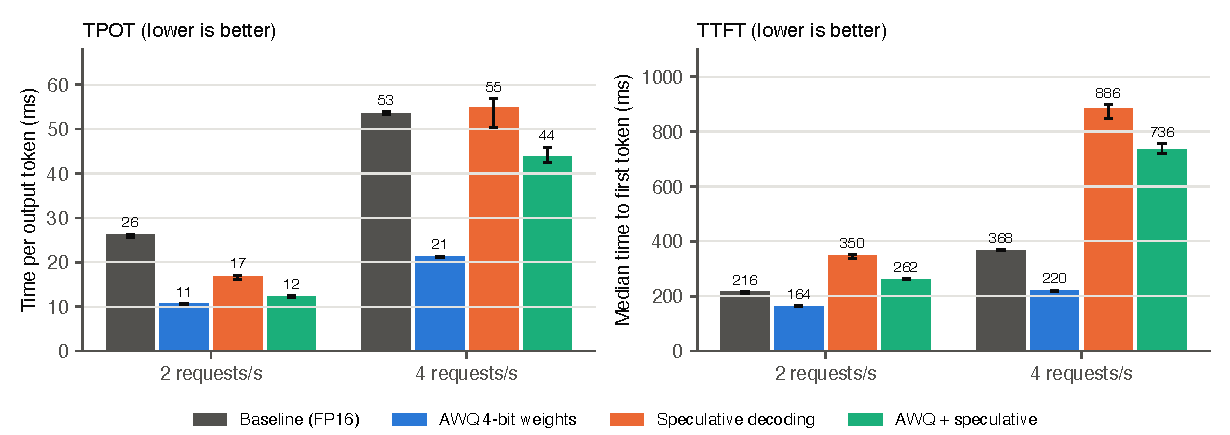
\includegraphics[width=.74\linewidth]{low_load.pdf}
\par\raggedright
\smallnote{Median of 4--6 runs; bars show the range. 1,024 prompt + 128 output tokens.}
\vspace{.05cm}
\begin{points}
\item AWQ: 2.5$\times$ lower TPOT (26 $\rightarrow$ 11 ms) and lower TTFT at both loads.
\item Speculative decoding: 1.6$\times$ lower TPOT at 2 requests/s, none at 4; higher TTFT at both.
\end{points}
\end{frame}

\begin{frame}{Contribution of each technique}
\smallnote{TPOT speed-up over the FP16 baseline (higher is better); TTFT change in brackets.}
\centering
\begin{tabular}{@{}lccc@{}}
\toprule
Configuration & 2 requests/s & 4 requests/s & Overloaded, 16--64/s\\
\midrule
Baseline (FP16, vLLM defaults) & 1.00$\times$ & 1.00$\times$ & 4.0 requests/s served\\
\textbf{AWQ} & \textbf{2.47$\times$} (TTFT $-$24\%) & \textbf{2.52$\times$} (TTFT $-$40\%) & 4.0\\
Speculative decoding & 1.56$\times$ (TTFT $+$61\%) & 0.98$\times$ (TTFT $+$141\%) & \textbf{4.4} ($+$11\%)\\
AWQ + speculative & 2.11$\times$ (TTFT $+$21\%) & 1.22$\times$ (TTFT $+$100\%) & 4.4\\
\bottomrule
\end{tabular}\par\raggedright
\vspace{.2cm}
\begin{points}
\item AWQ alone (2.5$\times$) beats AWQ with speculation (2.1$\times$ and 1.2$\times$). With AWQ each 3B pass is cheap, so 5 draft steps cost more than they save; 55\% of drafted tokens are accepted.
\item Speculation stops paying between 2 and 4 requests/s. When overloaded it adds 11\% throughput, but TTFT is over a minute anyway.
\end{points}
\end{frame}

\begin{frame}{Status}
\begin{tabularx}{\linewidth}{@{}P{2.6cm}P{3.0cm}X@{}}
\toprule
Item & Status & Note\\
\midrule
M1: AWQ & \textbf{Done} & 2.5$\times$ lower TPOT below 4 requests/s; quality not measured\\
M1: FP8 KV cache & Blocked & Needs CUDA toolkit\\
M1: batching & Not started & Single GPU, so no sharding question\\
M2: speculative decoding & \textbf{Done} & Break-even between 2 and 4 requests/s\\
M2: prefix caching & Next & Needs prompts with shared prefixes\\
M3: attribution & First version & One prompt length only\\
\bottomrule
\end{tabularx}\par
\vspace{.15cm}
\begin{points}
\item Below the limit, AWQ alone was the best setup we tested. Speculative decoding helps only at light load.
\end{points}
\end{frame}

\begin{frame}{Limitations and next steps}
\begin{points}
\item \textbf{Limitations:} one prompt length (1,024 tokens); no shared prefixes; open-loop load far past capacity; AWQ quality not checked; one GPU, one model size.
\end{points}
\vspace{.1cm}
\centering
\begin{tabularx}{\linewidth}{@{}XXX@{}}
\toprule
Next two weeks & Then & Before the final review\\
\midrule
Prompt lengths 512--6,144 & Fixed-concurrency sweep & Attribution across regimes\\
Prefix caching off vs.\ on, shared prefixes & 2--3 draft tokens; other drafters & Best setup per regime\\
CUDA toolkit; FP8 KV cache & Goodput at latency target & Profiling of the limit\\
AWQ quality on a small benchmark & Batch-size and scheduling tuning & Final plots and scripts\\
\bottomrule
\end{tabularx}\par
\vspace{.15cm}
\raggedright
\begin{points}
\item \textbf{Latency target (M1):} TTFT under 1 s and TPOT under 50 ms, reported as goodput (requests/s meeting both).
\end{points}
\end{frame}

\begin{frame}[plain,c]
\vfill
\begin{center}
{\LARGE\bfseries Thank You\par}
\end{center}
\vfill
\end{frame}
\end{document}
